%%==========SETUP===========%%
\documentclass{elsinta}
\usepackage{array}
\usepackage{booktabs}

% --- Memasukkan Data Dokumen Menggunakan ---
\projectcode{EL1}
\documentname{\ProjectProposalTitle} 
\documenttitle{Teknik Elektro - Sistem Informasi Tugas Akhir}
\capstonetitle{Monitoring on Induction Motor in Real-Time: Vibration and Temperature}
\shortname{MONTREAL-VT} 
\documentnumber{TA2526.02.003}
\revisionnumber{02}
\publicationdate{2 September 2026}
\revdatefooter{2/9/2026}

% --- Memasukkan Data Halaman Pengesahan (Halaman 2) ---
\currentpage{2} % Halaman yang sedang dicetak
% Data Tim
%Mahasiswa 1
\ketuatimnama{Mahasiswa 1}
\ketuatimnim{121130027}
%Mahasiswa 2
\anggotanamaI{Mahasiswa 2}
\anggotanimI{12345678}
%Mahasiswa 3
\anggotanamaII{Mahasiswa 3}
\anggotanimII{12345678}
% Data Dosen
%Pembimbing 1
\pembimbingInama{Dosen 1}
\pembimbingInip{12345678 123456 1 123}
%Pembimbing 2
\pembimbingIInama{Dosen 2}
\pembimbingIInip{12345678 123456 1 123}
% Tanggal Pengesahan
\approvaldate{27 April 2026}

\begin{document}

% Panggil perintah untuk membuat halaman sampul
\coverpage
% Pindah ke Halaman Baru
\newpage

% % Membuat Halaman Pengesahan (Halaman 2)
% \approvalpage

% % Lanjut ke halaman proposal
% \newpage

% ======================================
% Bagian Konten Proposal Dimulai di Sini
% ======================================

% Mengatur ulang nomor halaman dan gaya halaman
\clearpage
\pagenumbering{arabic}
\setcounter{page}{1} 
\pagestyle{myfooter} % Ganti dari 'plain' ke 'myfooter'

% Atur margin standar (Opsional, jika Anda ingin margin isi berbeda dari sampul)
% \newgeometry{left=4cm, right=3cm, top=3cm, bottom=3cm} 
% Catatan: Perintah \newgeometry memerlukan paket 'geometry' yang sudah ada di cls.

\cleardoublepage % Memastikan Daftar Isi dimulai di halaman kanan (jika menggunakan two-side)
\phantomsection % Penting untuk hyperref agar link Daftar Isi menunjuk ke halaman yang benar

%%=============DAFTAR ISI===============%%
\tableofcontents

%%=============SUMMARY=================%%
\newpage
\section*{\docsumary}
%%----Document Summary merupakan ringkasan yang hanya membahas isi dari dokumen capstone yang sedang dikerjakan, bukan keseluruhan proyek capstone. Bagian ini menjelaskan secara singkat tujuan, ruang lingkup, dan pokok pembahasan dari dokumen tersebut. Misalnya, pada dokumen EL1, ringkasan berfokus pada latar belakang, identifikasi masalah, dan lain-lain sesuai isi dari EL1.  Penulisan dilakukan secara padat dan jelas agar pembaca dapat langsung memahami inti dari dokumen tersebut tanpa mengaitkannya dengan bagian atau dokumen capstone lainnya.
% Topik yang dibahas pada EL100 dalam proyek "\textbf{Sistem Monitoring Getaran dan Suhu Motor Induksi untuk Prediksi Kerusakan (Predictive Maintenance)}" mencakup rencana pengembangan sistem pemantauan kondisi motor berbasis parameter getaran dan suhu sebagai bagian dari implementasi dari \textit{predictive maintenance}. Pengembangan sistem ini dilatarbelakangi pada tingginya persentase penggunaan motor induksi di sektor industri ($\approx 85\%$ penggunaan industri) serta risiko kerusakan yang dapat menyebabkan \textit{downtime} dan kerugian ekonomi akibat pemberhentian proses produksi apabila proses pemeliharaan dilaksanakan pasca kerusakan. 
% Proyek ini dilakukan guna merancang dan mengimplementasikan sistem pemantauan berbasis sensor getaran dan suhu yang mampu melakukan akuisisi data secara \textit{real-time}, serta terintegrasi IoT untuk visualisasi data dan pemantauan jarak jauh. Sistem pemantauan motor ini dirancang agar mampu memberikan indikasi kondisi motor dan rekomendasi tindakan pemeliharaan berdasarkan algoritma yang sudah diprogram. Selain itu, proyek ini memiliki tujuan tambahan mencakup analisis tren parameter sebagai indikator degradasi motor serta evaluasi efektivitas parameter sebagai indikator degradasi serta evaluasi efektivitas parameter getaran dan suhu dalam mendeteksi kondisi tidak normal pada motor.
% Proyek ini mencakup perancangan perangkat keras dan perangkat lunak sistem pemantauan yang mampu bekerja secara \textit{real-time} dengan integrasi IoT. Namun, proyek ini memiliki tetapan batasan yang meliputi batasan anggaran, pengoperasian pada kondisi suhu ruang, fokus pada deteksi kerusakan mekanis dan anomali termal, serta sistem tidak diberi otoritas untuk melakukan tindak pemeliharaan ter-otomasi.
% Dari sisi analisis bisnis, proyek ini menargetkan institusi pendidikan, terutama yang berfokus pada bidang teknologi, industri berbasis motor induksi, serta UMKM di bidang reparasi motor listrik. Kebutuhan pasar yang belum terpenuhi mencakup ketersediaan sistem pemantauan motor induksi dengan biaya instalasi rendah, sistem yang mudah diimplementasikan pengguna, serta sistem yang mampu memberikan informasi diagnostik yang sederhana dan dapat dipahami. Oleh karena itu, proyek ini menawarkan proposisi nilai berupa sistem pemantauan yang ekonomis, terintegrasi, dan aplikatif untuk meningkatkan keandalan operasi motor induksi.

Dokumen ini membahas mengenai latar belakang atas
perancangan sistem pemantauan kondisi motor induksi
dengan nama proyek \textbf{Monitoring On Induction Motor In Real-Time: Vibration and Temperature
(MONTREAL-VT)}.

Motor Induksi merupakan mesin listrik yang umum
digunakan pada proses produksi dan manufaktur.
Cakupan penggunaan motor induksi mencakup 85\% dari
total penggunaan motor pada pabrik dan operasi manufaktur.
Oleh karena itu, pemantauan kondisi motor induksi sangat penting
untuk dilakukan untuk mencegah adanya kerusakan yang tidak terprediksi. Parameter getaran
dipilih sebagai opsi parameter utama karena memiliki korelasi yang tinggi terhadap kerusakan mekanis pada motor induksi.
Di sisi lain, parameter arus, suhu, dan RPM dipilih sebagai parameter yang ditujukan untuk mendeteksi
adanya kerusakan elektrik dan sebagai unit proteksi pada motor.

MONTREAL-VT menawarkan solusi pemantauan kondisi motor induksi yang ekonomis, terintegrasi, dan 
aplikatif untuk meningkatkan keandalan operasi motor induksi sehingga
elemen UMKM dan industri skala kecil mampu mengimplementasikan
pemantauan kondisi motor untuk mendukung efisiensi produksi.

%===============BAB 1===================%
\newpage
\section{\BackgroundTitle}
\subsection{\NeedTitle}
Motor induksi merupakan jenis motor listrik arus bolak-balik yang umum digunakan dalam keseharian, industri dan domestik. Cakupan penggunaan motor induksi mencapai 85\% dari total penggunaan motor pada pabrik dan operasi manufaktur \cite{Ayankoso2026}. Hal ini disebabkan oleh biaya operasi  motor induksi yang rendah, struktur motor yang kokoh, dan keandalan tinggi sehingga motor induksi secara umum dapat diaplikasikan sebagai konveyor, \textit{crane}, kompresor, dan pompa \cite{Kumar2019,Gangsar2020}.  % Dalam implementasinya, motor induksi yang umum dipakai adalah motor induksi 3-fasa dan 1-fasa. 

\begin{figure}[b!]
    \centering
    \label{fig:faults_ieee}
    \begin{minipage}[b]{0.48\textwidth}
        \centering
        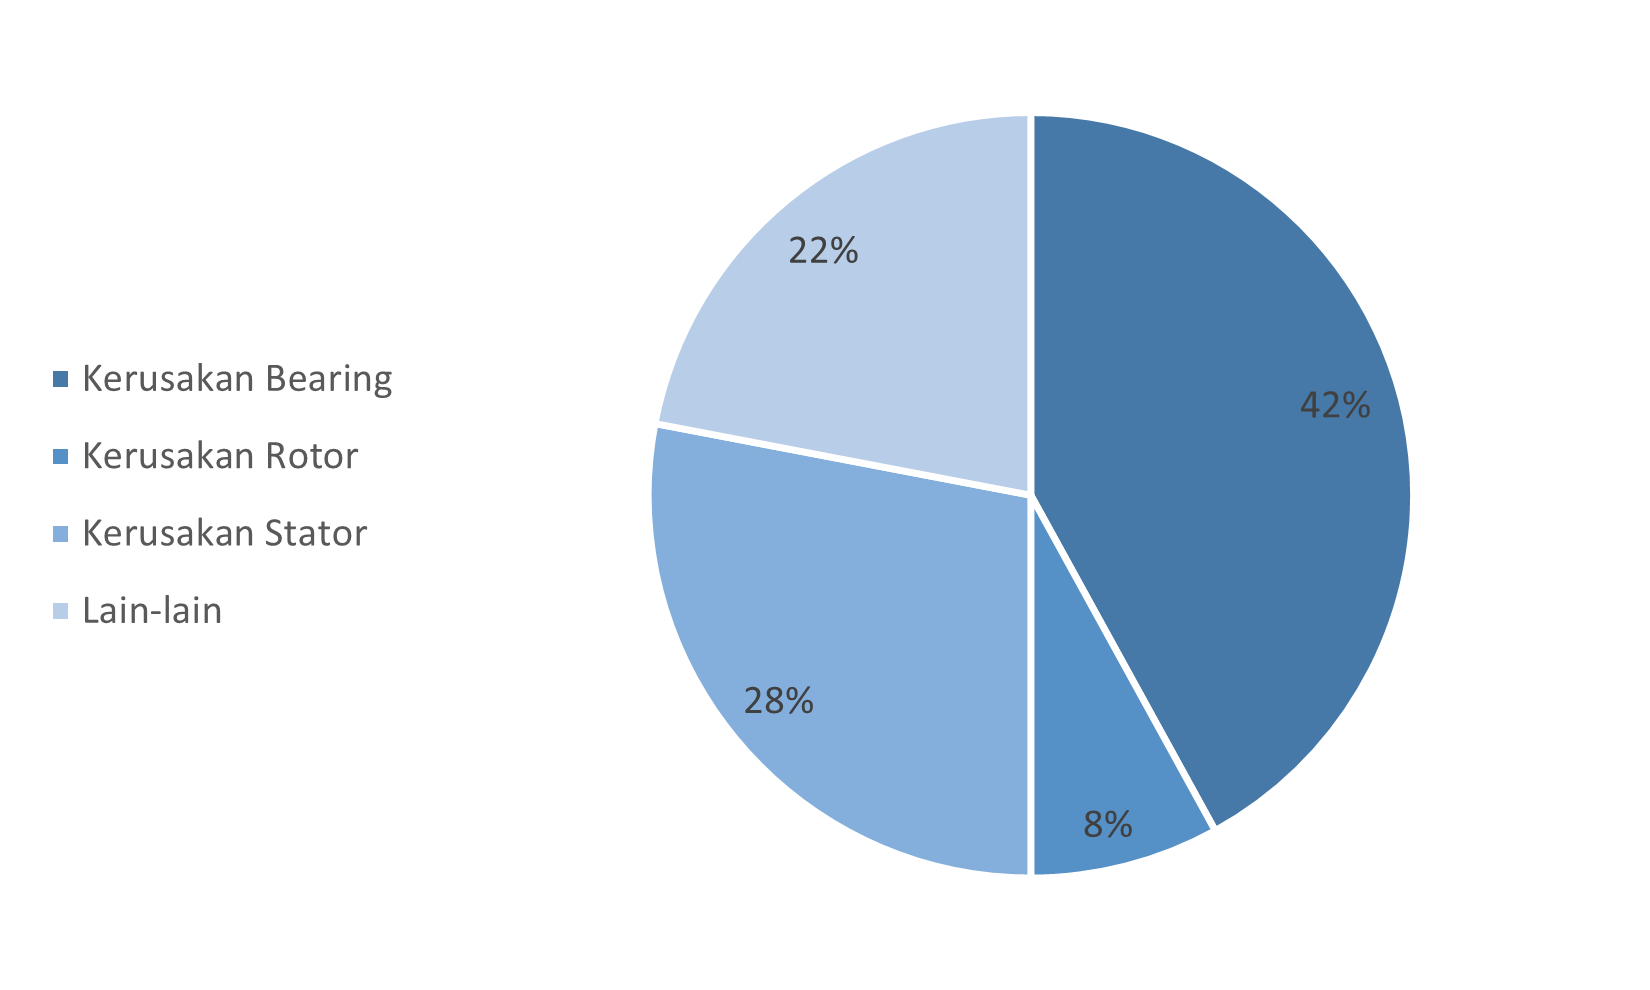
\includegraphics[width=\textwidth]{image/doc/motor-faults-ieee.png}
        \caption{Studi kasus IEEE-IGA mengenai komponen vital motor induksi \cite{Gundewar2020}}
        \label{fig:induction_motor_ieee}
    \end{minipage}
    \hfill
    \begin{minipage}[b]{0.48\textwidth}
        \centering
        \label{fig:faults_epri}
        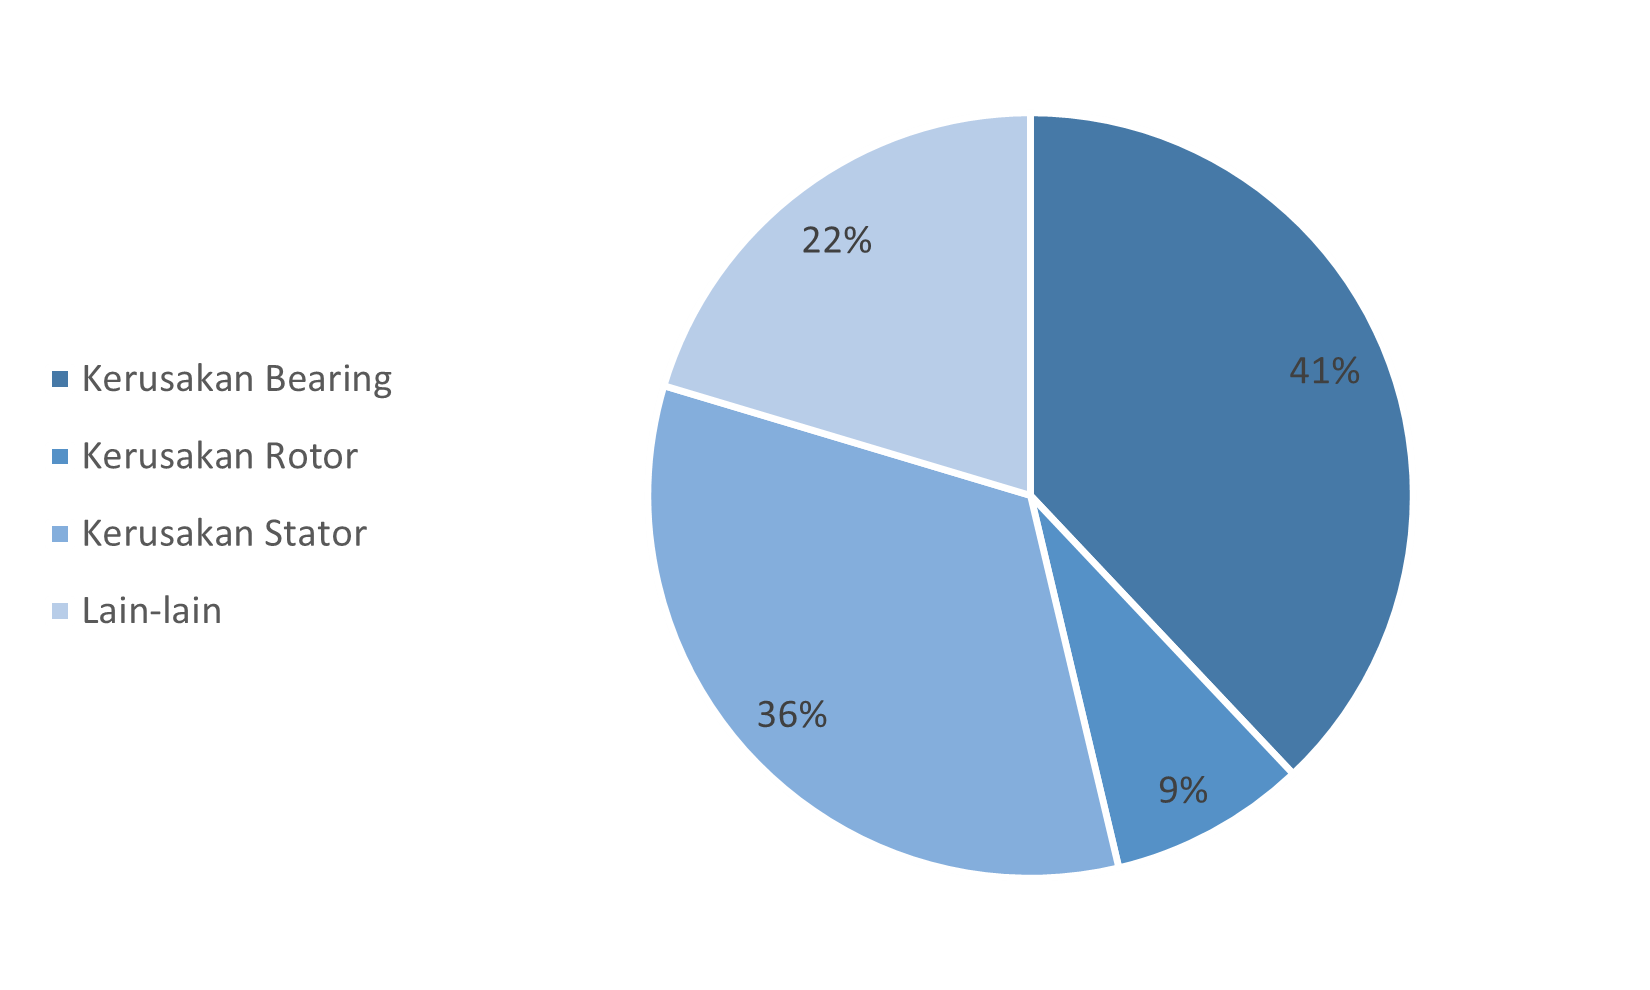
\includegraphics[width=\textwidth]{image/doc/motor-faults-epri.png}
        \caption{Studi kasus EPRI mengenai komponen vital motor induksi \cite{Gundewar2020}}
        \label{fig:induction_motor_epri}
    \end{minipage}
\end{figure}

Menurut Kumar et al. \cite{Kumar2019}, 
kerusakan pada motor induksi dapat 
disederhanakan menjadi kerusakan bagian motor 
yang meliputi bearing, stator, rotor, dan 
lain-lain (kumparan dan laminasi, rangkaian 
magnetik, dielektrik) yang persentase kerusakannya
ditunjukkan oleh grafik pada gambar \ref{fig:faults_ieee}
dan \ref{fig:faults_epri}. Kedua gambar tersebut 
menunjukkan bahwa tipe kerusakan mekanis adalah
tipe kerusakan yang lebih umum dijumpai pada 
motor induksi. Maka dari itu, parameter
yang harus diutamakan dalam pemantauan kondisi motor
induksi adalah parameter yang sensitif terhadap
kerusakan mekanis.

Pendekatan pemantauan kondisi motor menjadi 
solusi yang relevan sebagai upaya pemeliharaan 
prediktif (PdM). Pemantauan kondisi motor 
bertujuan untuk mengevaluasi keadaan performa 
dan kesehatan motor\cite{Mystkowski2022}, 
dan peralatan \cite{Nithin2022}. 
Proses pemantauan motor dapat dilakukan dengan 
berfokus pada beberapa parameter 
yang meliputi; suhu winding, getaran shaft, \textit{noise}, 
rus winding, tegangan \cite{VishnuKvAnoopBk2015}. 
Akan tetapi, tidak seluruh jenis parameter 
memiliki korelasi yang tinggi terhadap 
kerusakan motor. Parameter getaran dan suhu 
merupakan indikator yang paling signifikan 
dalam mendeteksi ketidaknormalan pada kinerja 
motor \cite{Filho2025}. Namun, parameter
getaran lebih sensitif terhadap kerusakan mekanis
dibandingkan parameter arus\cite{Ayankoso2026}.

%Parameter suhu
Di sisi lain, parameter arus dapat dimanfaatkan untuk
mendeteksi adanya kerusakan elektrik pada motor.
Urgensi atas deteksi kerusakan elektrik adalah
karena jenis kerusakan elektrik memiliki porsi sebesar
45\% dari seluruh kerusakan motor\cite{Filho2025}.
Kerusakan elektrik umumnya mengakibatkan kenaikan suhu
pada winding \cite{Filho2025}. Lonjakan
arus pada winding motor mengakibatkan kenaikan suhu pada
winding motor\cite{Filho2025}. Selain itu,
parameter suhu dapat dimanfaatkan sebagai
upaya proteksi pada winding motor untuk mencegah
\textit{Thermal overload}\cite{Gedzurs2015}.


Dengan demikian, pengembangan sistem pemantauan
kondisi berbasis parameter getaran dan suhu 
tidak hanya relevan, melainkan menjadi 
kebutuhan dalam meningkatkan keandalan dan 
keberlanjutan operasional sistem produksi 
berbasis motor induksi, khususnya dalam 
aplikasi industri yang menuntut keberlanjutan 
dan efisiensi yang tinggi.

%%===============Diagram 5 Why=================%%
    \usetikzlibrary{positioning}
    \begin{figure}[t!]
    \centering
    
    \begin{tikzpicture}[
    node distance=0.5cm,
    box/.style={
    draw,
    rectangle,
    rounded corners,
    align=center,
    text width=15cm,
    minimum height=0.5cm
    },
    arrow/.style={->, thick}
    ]
    
    \node[box] (A) at (0,0)
    {\textbf{Masalah Utama}\\
    Sistem pemantauan kondisi motor induksi tidak mampu dijangkau
    elemen UMKM dan industri skala kecil karena terlalu mahal};
    
    \node[box, below=of A] (B)
    {\textbf{WHY 1}\\
    Elemen UMKM dan industri skala kecil tidak memiliki akses terhadap
    sistem pemantauan kondisi motor induksi};
    
    \node[box, below=of B] (C)
    {\textbf{WHY 2}\\
    Pemantauan kondisi motor induksi dilakukan dengan cara manual};
    
    \node[box, below=of C] (D)
    {\textbf{WHY 3}\\
    Pemeriksaan kondisi motor secara manual
    kurang efisien dan memiliki risiko kecelakaan
    pada tingkat tertentu.};
    
    \node[box, below=of D] (E)
    {\textbf{WHY 4}\\
    Pemeriksaan yang kurang efisien dan berbahaya
    dapat mengakibatkan risiko kerusakan motor meningkat};
    
    \node[box, below=of E] (F)
    {\textbf{Akar Masalah}\\
    Pemeriksaan kondisi motor induksi
    yang dilakukan secara manual dapat mengakibatkan
    risiko kerusakan motor yang meningkat dan menyebabkan
    kerugian ekonomi akibat \textit{downtime} motor.};
    
    \draw[arrow] (A) -- (B);
    \draw[arrow] (B) -- (C);
    \draw[arrow] (C) -- (D);
    \draw[arrow] (D) -- (E);
    \draw[arrow] (E) -- (F);
    
    \end{tikzpicture}
    
    \caption{Diagram Analisis 5 Why}
    
    \end{figure}
%%===========End Diagram 5 Whys==================%%

\subsection{\ExistingConditionTitle}
Beberapa strategi pemeliharaan mesin yang diketahui secara umum meliputi \textit{preventive maintenance}, \textit{predictive maintenance}, \textit{corrective maintenance}, \textit{reliability maintenance} dan total \textit{productive maintenance}\cite{Nithin2022,Hassan2024}. Preventive maintenance umum diaplikasikan di dunia industri manufaktur, transportasi, dan energi, memastikan prosedur pemeliharaan dilaksanakan secara terjadwal sehingga mampu memaksimalkan umur penggunaan mesin, mengurangi kegagalan mesin yang merugikan, dan menjamin keandalan\cite{Tsunashima2019}.

Tindakan PdM pada motor induksi berdasarkan jenis kerusakan dapat diklasifikasikan menjadi \textit{electrical predictive maintenance}  (E-PdM) dan \textit{mechanical predictive maintenance} (M-PdM). \textit{electrical predictive maintenance} meliputi \textit{motor current signature analysis} (MCSA), dan \textit{instantaneous power signature analysis} (IPSA) \cite{Venkatesh2022}. Lebih lanjut, tindak \textit{mechanical predictive maintenance} yang umum diaplikasikan meliputi \textit{vibration analysis technique} (VAT), \textit{acoustic analysis}, and \textit{speed oscillations}\cite{Venkatesh2022}. 

M-PdM umum dilakukan untuk mendeteksi kerusakan pada sistem mekanis motor seperti kerusakan bearing, ketidakselarasan dan ketidakseimbangan komponen mekanis, serta komponen longgar. VAT merupakan salah satu metode pemantauan kondisi mekanis motor dengan tujuan menjadikan getaran motor sebagai parameter ukur dengan memanfaatkan accelerometer sebagai sensor. VAT memiliki tingkat korelasi yang tinggi terhadap indikasi kerusakan mekanis pad motor induksi \cite{Pardeshi2022}. Metode lain yang umum dipakai adalah \textit{acoustic signature} dengan memanfaatkan data suara mesin yang diubah domainnya dengan \textit{fast-fourier transform} (FFT) \cite{Venkatesh2022,Sonowal2019}.

MCSA merupakan metode E-PdM dengan menggunakan arus sebagai parameter ukur. MCSA pada umumnya dipakai karena biaya rancangan yang rendah, \textit{current clamps} dan tranduser tertanam pada feeder motor. Ranah aplikasi MCSA umumnya tidak berbeda dari VAT, dengan kelebihan pemantauan parameter lonjakan arus pada motor \cite{Cameron1986}. Praktik MCSA pada industri tidak akan mengganggu produktivitas industri karena bersifat non-intrusif, artinya proses pemantauan tidak mengharuskan pemberhentian operasi motor \cite{Venkatesh2022}.

Parameter lain yang layak dipertimbangkan sebagai alasan penguat tindakan pemeliharaan motor adalah suhu. Suhu tinggi pada motor induksi umumnya mampu mengidentifikasikan kerusakan kumparan pada stator, atau beban berlebih \cite{Filho2025}. Pengukuran suhu umumnya dilakukan dengan menggunakan \textit{thermocouple} yang ditempatkan pada bagian motor yang telah ditentukan, biasanya bagian internal, enclosure, frontal bearing, end bracket \cite{Filho2025}. Hal ini disebabkan penggunaan alat lain seperti sensor \textit{infra-red}, hanya secara realistis diimplementasikan untuk mengetahui suhu motor dari sisi eksternal \cite{Mahami2021}. Perbandingan performa masing-masing metode dan parameter tercantum pada tabel EL1.1.


% Source - https://tex.stackexchange.com/a/22861
% Posted by Stefan Kottwitz, modified by community. See post 'Timeline' for change history
% Retrieved 2026-03-23, License - CC BY-SA 4.0

%%===============Tabel Perbandingan Metode dan Parameter Pemantauan==============%%
\begin{table}[t!]
\centering
\caption{Perbandingan parameter uji pada motor induksi}
\begin{tabular}{|p{2cm}|p{3cm}|p{4cm}|p{4cm}|}
\hline
\textbf{Ref.} & \textbf{Metode} & \textbf{Aplikasi} & \textbf{Efektivitas}\\ \hline

%baris 1
Ul Hassan et al. \cite{Hassan2024}, Pardeshi et al. \cite{Pardeshi2022} 
& \textit{Vibration analysis technique} (VAT).
& Kerusakan mekanis; ketidakselaran, ketidakseimbangan, kerusakan bearing,  komponen longgar.
& Efisien biaya, non, intrusif, korelasi tinggi terhadap kerusakan mekanis.\\ \hline

%baris 2
Cameron et al. \cite{Cameron1986}
& \textit{Motor current signature analysis} (MCSA).
& Kerusakan elektrik dan mekanis; rotor bar patah, \textit{air-gap eccentricity}, short-circuit.
& Efisien biaya, non-intrusif.\\ \hline

%baris 3
Filho et al. \cite{Filho2025}, Lee et al. \cite{Lee2002}
& Suhu (Thermocouple)
& Overload, pemanasan kumparan stator .
& Pemantauan suhu secara fisik pada bagian motor.\\ \hline

%baris 4
Mahami et al. \cite{Mahami2021}
& Suhu (Infra-red)
& Titik pemanasan, kebocoran insulasi.
& Pengawasan visual langsung.\\ \hline

%baris 5
Venkatesh et al. \cite{Venkatesh2022}
& \textit{Acoustic Signature}
& Kerusakan rotor/bearing, ketidakserasian komponen.
& Tingkat akurasi tinggi, biaya murah.\\ \hline

\end{tabular}
\end{table}

\subsection{\ProjectUrgencyTitle}
% Di bagian ini dijelaskan mengapa proyek capstone perlu segera dilakukan. Penekanan dapat diberikan pada masalah yang semakin mendesak, peluang yang akan hilang jika tidak dimanfaatkan, atau dampak negatif jika permasalahan tidak segera diatasi. Subbab ini juga bisa menekankan manfaat strategis, baik untuk pengembangan ilmu, teknologi, maupun aplikasi praktis yang dapat dirasakan oleh pengguna.
\begin{enumerate}
    \item Sistem pemantauan kondisi pada motor induksi merupakan komponen dasar dalam upaya PdM dalam operasi industri. Sistem ini memungkinkan evaluasi kondisi mesin secara kontinu melalui parameter operasional seperti getaran, suhu, dan arus. Sistem pemantauan ini berfungsi sebagai tolak ukur keandalan motor listrik dijaga dalam kondisi optimal.
    \item Kebutuhan sistem peringatan dini (early fault detection) dalam sistem produksi yang semakin kritis, terutama dalam proses identifikasi degradasi performa motor induksi. Implemetasi sistem peringatan dini memungkinkan tindakan pemeliharaan yang secara signifikan mampu menekan risiko downtime tidak terencana, mengurangi biaya perbaikan motor, serta meminimalkan tingkat kerugian.
    \item Aspek aksesibilitas dan efisiensi biaya menjadi pertimbangan utama dalam pengembangan sistem terutama untuk industri skala kecil dan menengah. Sistem pemantauan sederhana dengan biaya implementasi rendah mampu menjembatani kesenjangan teknologi pemantauan industri tingkat tinggi pada industri skala kecil.
    \item Kebutuhan akan sistem proteksi otomatis yang mencegah keadaan bahaya seperti overload, overcurrent, dan overheat pada motor induksi.
\end{enumerate}

\section{\ObjectivesTitle}

\subsection{\MainObjectiveTitle}
%Tujuan utama merupakan hasil inti dari proyek ini, menggambarkan sistem atau layanan yang akan dihasilkan, dengan indikator pencapaian yang terukur.    
\begin{enumerate}
  \item Mengembangkan sistem pemantauan kondisi 
  motor induksi dengan berbasis sensor getar, sensor suhu,
  sensor arus, dan sensor RPM. Sensor getaran
  harus mampu diimplementasikan pada \textit{vibration time-domain analysis},
  dan \textit{vibration frequency-domain 
  analysis} dengan metode \textit{frequency-signature analysis}.
  Metode \textit{envelope analysis} untuk mendeteksi
  kerusakan bearing apabila dimungkinkan.
  \item Mengembangkan sistem pemantauan kondisi
  dengan parameter suhu, arus dan \textit{Revolution per Minute} (RPM), dengan galat pengukuran pada parameter
  suhu dan arus tidak lebih dari 5\%. Parameter ini
  harus mampu diimplementasikan sebagai sistem proteksi motor.
  \item Mengembangkan sistem IoT terintegrasi Wi-Fi sebagai 
  media informasi dan komunikasi yang ramah 
  pengguna, yang mampu mengirim dan menampilkan
   data secara \textit{real-time} dengan 
   time-delay $\leq 1000ms$, serta diuji 
   melalui minimal 5 skenario penggunaan 
   pengguna.
%   \item Merancang dan membuat sistem pengendali
%    kecepatan motor induksi berbasis kontrol tertutup yang mampu menjaga kecepatan dengan \textit{error steady-state}, setpoint, waktu tunak yang tidak  melebihi batas ketetentuan, dan overshoot terkendali.
  \item Menyusun dokumentasi teknis dan manual pengguna yang membahas mengenai proses perancangan alat, penggunaan, serta data akuisisi sistem pemantauan motor induksi sehingga dapat digunakan, dikembangkan, atau direplikasi, dan diselesaikan bersamaan dengan selesainya perancangan alat. 
\end{enumerate}

\subsection{\AdditionalObjectivesTitle}
% Tujuan tambahan adalah target pendukung yang memperkuat keberhasilan proyek meskipun bukan keluaran inti, biasanya terkait dokumentasi, diseminasi, atau peningkatan kualitas sistem.
\begin{enumerate} 
    \item Mengimplementasikan enkripsi sistem IoT yang menjamin keamanan transmisi data dari sensor ke mikrokontroler dan dari mikrokontroler ke cloud.
    \item Merancang sistem analisis getaran dengan metode \textit{envelope analysis}
    untuk mendeteksi kerusakan bearing secara detil.
\end{enumerate}

\subsection{\DeliverablesTitle}

Luaran yang dihasilkan dari proyek ini mencakup beberapa keluaran utama yang mendukung tujuan utama dan tujuan tambahan, antara lain:

\begin{enumerate}
    \item \textbf{Prototipe sistem pemantauan yang terdiri atas sensor dan pengkondisian sinyal:} \\
    Sistem pemantauan getaran dan suhu motor 
    induksi yang mampu merekam data secara 
    \textit{real-time}, minim derau, dan terintegrasi dengan cloud.
    \item \textbf{Dashboard interaktif:} \\ 
    yang menampilkan tingkat kesehatan motor, 
    visualisasi 
    parameter pemantauan kondisi motor, indikasi potensi
    kerusakan dan saran tindakan pemeliharaan 
    induksi.
    \item \textbf{Sistem proteksi motor induksi:}\\
    Sistem proteksi yang terdiri atas sistem relay dan saklar darurat. Serta
    rangkaian penyearah tegangan 220VAC ke 5 VDC untuk suplai daya mikrokontroler.
    \item \textbf{Laporan teknis dan manual pengguna} \\
    Data hasil pengukuran sensor accelerometer, dan sensor suhu. Lebih lanjut, terdapat proses instalasi, pengoperasian, pemeliharaan prototipe, indikasi kerusakan dan saran tindakan pemeliharaan motor induksi dalam terdokumentasi dalam bentuk laporan.
\end{enumerate}

\section{\ScopeConstraintsTitle}
\subsection{\ScopeTitle}
% Bagian ini menjelaskan ruang lingkup proyek secara jelas, yaitu apa saja yang termasuk ke dalam cakupan proyek dan apa yang berada di luar cakupan. Penjelasan ini penting agar pembaca tidak memiliki ekspektasi yang keliru terhadap hasil yang akan dicapai.  
% Sebagai contoh, proyek ini hanya berfokus pada \textit{pemantauan} suhu dan kelembaban di rumah kaca. Proyek tidak mencakup pengembangan kontrol otomatis untuk pompa nutrisi atau sistem irigasi cerdas. Dengan demikian, batasan yang ditetapkan dapat memberikan kejelasan sekaligus menjaga proyek tetap realistis dan sesuai waktu yang tersedia.  
Proyek ini mencakup perancangan sistem pemantauan kondisi motor induksi satu fasa berbasis pengukuran tren getaran dan suhu. Perolehan akuisisi plot data getaran digunakan untuk mendeteksi kerusakan mekanis melalui analisis domain waktu dan domain frekuensi data getaran, sedangkan sensor suhu ditempatkan pada bagian winding atau bagian yang konduktif terhadap suhu winding untuk mendeteksi terjadinya \textit{overheating}. Sistem pemantauan ini diimplementasikan dalam bentuk prototipe yang mencakup mikrokontroler sebagai unit pemrosesan utama, sensor getar, serta sensor suhu. Proses akuisisi dan pengolahan data dilakukan secara \textit{real-time} dengan \textit{time-delay} $\leq 1000ms$, dan terintegrasi dengan dashboard pemantauan untuk visualisasi data. Selain itu, sistem dilengkapi dengan mekanisme peringatan dini serta rekomendasi tindak pemeliharaan berdasarkan kondisi yang terdeteksi.

\subsection{\ConstraintsTitle}
% Constraints adalah batasan-batasan yang diberikan oleh stakeholder kepada  tim dalam melaksanakan proyek. Keterbatasan ini dapat berupa waktu, sumber daya manusia, ketersediaan perangkat keras atau perangkat lunak, serta faktor eksternal lainnya.  

% Contoh constraints yang relevan meliputi:  
Batasan yang telah ditetapkan oleh pihak pengembang adalah sbb;
\begin{enumerate}
    \item Anggaran pengembangan sistem dibatasi maksimal sebesar Rp. 1.000.000,00, sehingga pemilihan opsi komponen dan metode implementasi harus disesuaikan dengan keterbatasan biaya tersebut.
    \item Sistem dirancang untuk digunakan pada motor induksi satu fasa.
\end{enumerate}

\section{\BusinessAnalysisTitle}

\subsection{\MarketNeedsTitle}
% \textit{Penjelasan: Identifikasi siapa pasar target utama Anda (misalnya, institusi akademik, laboratorium, UKM, atau rumah tangga dengan risiko kebocoran gas). Jelaskan masalah spesifik yang dihadapi segmen ini dan bagaimana Project ini secara spesifik memenuhi kebutuhan tersebut.}

\subsubsection*{Segmen Target Utama:}
\begin{enumerate}
    \item \textbf{Institusi Pendidikan dan Penelitian ($\text{ITERA}$):} Lab praktikum dan penelitian yang berfokus pada sistem kendali, diagnostik, dan pemeliharaan motor induksi satu fasa dan tiga fasa.
    \item \textbf{Perusahaan industri berbasis motor induksi:} Perusahaan yang memanfaatkan motor induksi sebagai mesin utama dalam proses produksi, sehingga memerlukan opsi alternatif sistem pemantauan kondisi untuk meningkatkan keandalan dan mengurangi downtime dengan biaya yang lebih rendah.
    \item \textbf{Usaha kecil atau UMKM di sektor reparasi kumparan motor:} Pelaku usaha yang bergerak di bidang perbaikan dan penggulungan ulang (rewinding) motor listrik, yang membutuhkan alat bantu diagnostik untuk identifikasi dan kerusakan motor.
\end{enumerate}

\subsubsection*{Kebutuhan pasar yang Belum Terpenuhi:}
\begin{enumerate}
    \item \textbf{Ketersediaan Solusi Berbiaya Rendah (Low-Cost System):} Perangkat pemantauan getaran industri standar seperti \textit{vibration analyzer} atau sensor piezoelektrik kelas industri memiliki harga yang sangat mahal. Pasar membutuhkan opsi alternatif sistem perangkat yang memiliki biaya terjangkau namun memiliki akurasi yang tepat.
    \item \textbf{Pemantauan Real-Time dan Kontinu:} Banyak industri masih mengandalkan pengecekan manual dalam upaya CM secara berkala. Industri membutuhkan sistem yang mampu melakukan pemantauan dengan operasi non-stop.
    % \item \textbf{Aksesibilitas Data Jarak Jauh (Integrasi IoT):} Dashboard berbasis web yang memungkinkan data getaran dan suhu dipantau oleh pengguna dari kantor atau ruang kontrol secara remote.
    \item \textbf{Sistem Peringatan Dini Sederhana (User-Friendly Alerts):} Pasar membutuhkan sistem yang tidak hanya memberi data mentah numerik, tetapi juga memberikan indikator status berdasarkan batas kerja normal motor sesuai standar yang berlaku.
\end{enumerate}

\subsection{\ValuePropTitle}
% \textit{Penjelasan: Proposisi nilai adalah pernyataan ringkas mengenai manfaat spesifik yang ditawarkan Project ini kepada target pasar. Jawablah pertanyaan: "Mengapa pelanggan harus memilih Project ini, bukan solusi yang lain?"}

% \textbf{Contoh Value Proposition} dari Project ELSINTA berpusat pada tiga pilar utama: \textbf{Keselamatan, Keterjangkauan, dan Kecerdasan Data}.

\begin{enumerate}
    \item \textbf{Efisiensi Biaya Dalam Upaya Pemantauan Motor Induksi:} Proyek ini menawarkan fungsionalitas pemantauan getaran dan suhu dengan biaya rancang yang jauh lebih rendah. Hal ini memungkinkan laboratorium dan UMKM mampu mengoperasikan sistem pemantauan motor induksi.
    \item \textbf{Pemantauan Real-Time Non-stop:} Sistem pemantauan motor induksi bekerja setiap detik dengan time-delay minimum. Sistem mampu memberikan notifikasi getaran atau kenaikan suhu di luar batas normal, sesuai ISO 20816, IEC 60034, dan ISO 13373. Hal ini mencegah downtime yang merugikan produksi.
    \item \textbf{Aksesibilitas Data Berbasis IoT:} Sistem terintegrasi dengan dashboard berbasis web yang mampu dioperasikan secara remote sehingga proses pemantauan bersifat fleksibel.
\end{enumerate}


\subsection{Pemangku Kepentingan}

Subbab ini mengidentifikasi pihak-pihak yang terlibat maupun terdampak dalam pengembangan sistem pemantauan getaran dan suhu motor induksi untuk predictive maintenance. Setiap pemangku kepentingan memiliki peran dan kontribusi yang berbeda dalam mendukung keberhasilan proyek.

\begin{longtable}{|p{5cm}|p{9cm}|}
\caption{Daftar Pemangku Kepentingan dan Kontribusi} \\
\hline
\textbf{Pemangku Kepentingan} & \textbf{Peran \& Kontribusi} \\
\hline
\endfirsthead

\hline
\textbf{Pemangku Kepentingan} & \textbf{Peran \& Kontribusi} \\
\hline
\endhead

Tim Mahasiswa (Ketua dan Anggota) &
\textbf{Peran:} Pelaksana utama proyek yang bertanggung jawab dalam perancangan, pengembangan, integrasi, dan pengujian sistem pemantauan. \newline
\textbf{Kontribusi:} Menyediakan waktu, tenaga, serta kemampuan teknis dalam bidang elektronika, pemrograman, dan pengolahan data sensor. \\
\hline

Dosen Pembimbing &
\textbf{Peran:} Pembimbing akademik yang memberikan arahan metodologi, validasi konsep, dan evaluasi hasil proyek. \newline
\textbf{Kontribusi:} Memberikan masukan teknis, koreksi desain, serta memastikan kesesuaian proyek dengan kaidah ilmiah dan standar akademik. \\
\hline

Program Studi Teknik Elektro ITERA &
\textbf{Peran:} Institusi penyelenggara yang menyediakan fasilitas dan dukungan akademik. \newline
\textbf{Kontribusi:} Menyediakan laboratorium, peralatan pendukung, serta lingkungan pengujian sistem yang mendukung proses pengembangan proyek. \\
\hline

Pengguna Akhir (Teknisi/Karyawan Industri atau Staf Laboratorium) &
\textbf{Peran:} Pengguna langsung sistem pemantauan serta penguji fungsional dalam kondisi nyata. \newline
\textbf{Kontribusi:} Memberikan umpan balik terkait kemudahan penggunaan (usability), keakuratan informasi, serta efektivitas sistem dalam mendukung pemeliharaan motor. \\
\hline

% Pihak Industri / Mitra (Jika Ada) &
% \textbf{Peran:} Mitra implementasi yang menyediakan studi kasus atau lingkungan aplikasi nyata. \newline
% \textbf{Kontribusi:} Memberikan data operasional motor induksi, kebutuhan sistem di lapangan, serta validasi performa sistem dalam kondisi industri. \\
% \hline

Penyedia Perangkat (Sensor dan Mikrokontroler) &
\textbf{Peran:} Penyedia komponen utama yang digunakan dalam sistem pemantauan. \newline
\textbf{Kontribusi:} Menyediakan perangkat seperti sensor getaran, sensor suhu, serta mikrokontroler yang menjadi inti dari sistem. \\
\hline

Pengembang Platform IoT / Software &
\textbf{Peran:} Penyedia platform untuk pengolahan dan visualisasi data. \newline
\textbf{Kontribusi:} Menyediakan layanan dashboard, penyimpanan data, dan sistem notifikasi yang mendukung pemantauan secara real-time. \\
\hline
% \textbf{Pengguna Akhir} (Misalnya: Staf Lab/Karyawan) &
% \textbf{Peran:} Penerima Manfaat Langsung \& Penguji Fungsional. Menggunakan ruangan yang dipasangi sistem.
% \newline
% \textbf{Kontribusi:} Memberikan \emph{feedback} tentang kemudahan penggunaan (usability) dan fungsionalitas sistem di lingkungan nyata. \\
% \hline
% \textbf{Pihak Sponsor/Penyedia Perangkat} (Jika ada) &
% \textbf{Peran:} Penyedia Sumber Daya (misalnya, dana, sensor, atau layanan cloud).
% \newline
% \textbf{Kontribusi:} Dukungan material (sensor gas, mikrokontroler) atau dukungan teknis spesifik. \\
%\hline
\end{longtable}

Pemangku kepentingan tersebut saling berperan dalam mendukung keberhasilan proyek, baik dari sisi pengembangan teknis, validasi akademik, hingga implementasi di lapangan. Keterlibatan pengguna akhir dan mitra industri menjadi faktor penting dalam memastikan bahwa sistem yang dikembangkan benar-benar sesuai dengan kebutuhan dan dapat diterapkan secara nyata.

\section{\ReferencesTitle}
% Daftar pustaka ditulis sesuai standar IEEE, sebaiknya gunakan Citation tools seperti Mendeley, Zotero dll.  
% Contoh format IEEE:  
\renewcommand{\refname}{}      % Hapus judul default "Pustaka"
\bibliographystyle{IEEEtran} % Menggunakan style sitasi IEEE
\bibliography{pustaka}    % Memanggil file pustaka.bib

\section{\AbbrevTitle}

% longtable tidak menggunakan lingkungan table[] di sekitarnya.
% Perintah \begin{longtable} langsung menggantikan \begin{table}\begin{tabular}
\begin{longtable}{|p{4cm}|p{11cm}|} % Lebar kolom ditetapkan agar teks wrap
    \caption{Daftar Singkatan (Abbreviations)} \label{tab:abbreviationsEL1} \\
    \hline
    \textbf{Abbreviation} & \textbf{Definition} \\
    \hline
    \endhead % Mengakhiri baris header yang akan diulang di setiap halaman
    
    \hline 
    \multicolumn{2}{|r|}{Lanjutan di halaman berikutnya...} \\ 
    \endfoot % Footer untuk semua halaman kecuali yang terakhir
    
    \hline
    \endlastfoot % Footer untuk halaman terakhir (kosong)

    % --- Isi Tabel ---
    PdM & Predictive Maintenance \\
    \hline
    M-PdM & Mechanical Predictive Maintenance \\
    \hline
    E-PdM & Electrical Predictive Maintenance \\
    \hline
    VAT & Vibration Analysis Technique \\
    \hline
    MCSA & Motor Current Signature Analysis \\
    \hline    
    % Tambahkan lebih banyak baris di sini untuk memicu pemisahan halaman
    % ... (Tambahkan entri lain jika tabel perlu memanjang)

\end{longtable}

% Tambahkan \newpage jika Anda ingin halaman isi dimulai di halaman berikutnya
% \newpage
% \section*{Pendahuluan}
% Di sinilah konten proposal Anda akan dimulai...

\end{document}